\section{Results and Discussion} 
\label{sec:Results & Discussion}

\subsection{Channel Flow Results}



%%%%%%%%%%%%%%%%%%%%%%%%%%%%%%%%%%%%%%%%%%%%%%%%%%%%%%%%%%%%%%%%%%%%%%%%%%%%%%%%%%%%%%%%%%%%%%%%%%%%%%%%%%%%%%%%%%%%%%%%%%%%%%%%%%%%%%%%%%%%%%%%%%%%%%%%%%%%%%%%%%%%%%%%%%%%%%%%%%%%%%%%%%%%%%%%%%%%%%%%%%%%%%%%%%%%%%%%%%%%%%%%%%%%%%%%%%%%%%%%%%%%%%%%%%%%%%%%%%%%%%%%%%%%%%

\subsubsection{Grid Convergence Study and Generalised Richardson Extrapolation Result}
A parameter of the simulation results is used to determine the ideal and converged simulation result using the Generalised Richardson Extrapolation. Coefficient of friction parameter in various resolutions are used in the grid convergence study, with the results shown in the Figure \ref{sec:Computational procedures}.

\begin{figure}[h!]
	\centering
	\label{fig:GREP_res}
	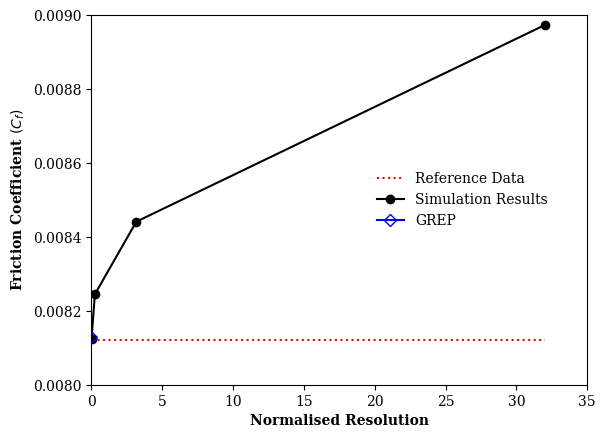
\includegraphics[width=0.75\linewidth]{Figures/GCS_real}
	\caption{Grid Convergence Study with Generalised Richardson Extrapolation}
\end{figure}

Based on the results, it is apparent that the resolution values are already sufficient to show a converging value in the channel flow simulations. Additionally, the value is converging to the reference data given \cite{Lee_Moser_2015}. with the fine resolution already quite close the reference data. This is a promising result as it can suggest that the fine resolution values are adequate to simulate channel flows at $Re_\tau = 180$, decreasing the computational requirement.

For the Generalised Richardson extrapolation, the result is nearly identical to the reference data and the finest mesh resolution, only yields to 0.00093 \% difference to the reference value and 0.00046 \% error to the finest mesh resolution. Therefore, the proposed Generalised Richardson Extrapolation can be deemed as valid and sufficient model to predict the values of channel flow simulation in an idealised state.

\subsubsection{Mean Streamwise Velocity}
\label{sec:XVelo}
Figure \ref{fig:upyp} displays the mean streamwise velocity of the channel flow normalised to the viscous length scale. The result is as expected, as the value of the velocities becomes closer to the reference data \cite{Lee_Moser_2015}.
\begin{figure}[h!]
	\centering
	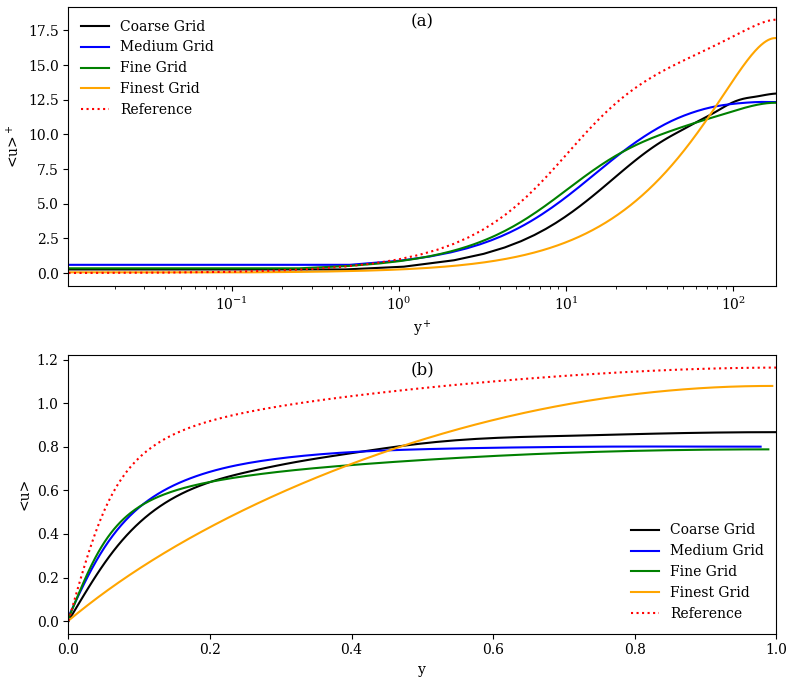
\includegraphics[width=0.9\linewidth]{Figures/upyp}
	\caption[Mean Streamwise Velocity]{Mean Streamwise Velocity (a) as a Function of Viscous Length Scale and (b) As It Is, on the First Half of the Height of the Channel Flow. The Reference Data Corresponds with Lee and Moser Channel Flow Data~\cite{Lee_Moser_2015}}
	\label{fig:upyp}
\end{figure}

The finest mesh model is the only mesh model that has values close to the reference values, showing only 1.02\% difference on the maximum velocity. However, in the overall values, the finest mesh models displays different trend of of streamwise velocity compared to the other mesh models, as well as the reference values. The difference can be understood by analysing the streamwise velocity profile changes in the channel flow, shown in Figure \ref{fig:chanflowveloprof}.

\pagebreak

\begin{figure}[h!]
	\centering
	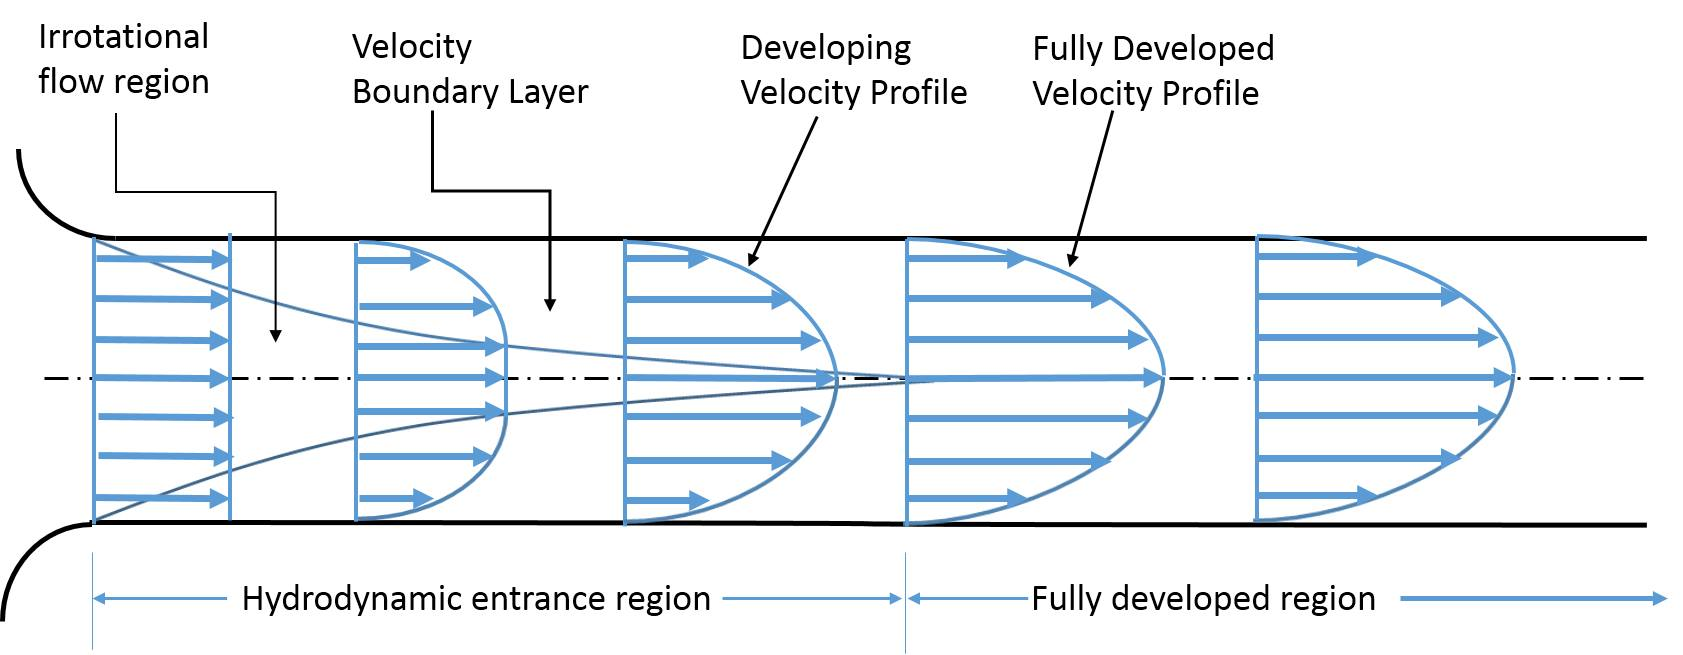
\includegraphics[width=0.9\linewidth]{Figures/chanflowveloprof}
	\caption[Streamwise Velocity Changes in a Channel Flow]{Streamwise Velocity Profile Changes in a Channel Flow~\cite{Cengel2019}}
	\label{fig:chanflowveloprof}
\end{figure}


 The finest mesh models shows a fully developed velocity profile, while the other models shows a velocity trend that mimics a flow with developing boundary layers. This is caused by the long iteration time. This gives the boundary layer more time to fully develop, thus gives the different trend of velocity profile.




\subsubsection{Reynolds Stresses}
\label{sec:Reystress}



\subsubsection{Velocity Distribution}
\label{sec:Flow physics}


\subsubsection{Pressure and Moment Coefficients}
\label{sec:Pressure coefficient}



\subsection{Viscous Flow}
\label{sec:ViscFlow}



\subsection{Off-Design Conditions}
\label{sec:ODC}


